% ============================================================
% experiments/exp01_smoke/report.tex
% exp01_smoke 实验报告 —— 自包含「实验设置 + 正确性用例 + OD 结果 + 图件」
%
% 数据来源（路径均相对本文件）：
%   results/metrics.json      全部数值指标（本文数字均出自该文件）
%   results/figures/          图件 5 张（fig_region_overview / fig_overview /
%                             fig_route_vs_path / fig_trajectory / fig_side_view）
%
% 编译：latexmk -xelatex report.tex     （ctex 需 xelatex）
% ============================================================
\documentclass[a4paper,11pt]{article}

\usepackage[margin=2.3cm]{geometry}
\usepackage{graphicx}
\usepackage{booktabs}
\usepackage{caption}
\usepackage{float}
\usepackage{amsmath,amssymb}
\usepackage{array}
\usepackage[table]{xcolor}
\usepackage[hidelinks]{hyperref}
\usepackage{ctex}

\graphicspath{{results/figures/}}

\captionsetup{font=small,labelfont=bf,skip=6pt}
\setlength{\parskip}{4pt}
\renewcommand{\arraystretch}{1.15}
\setlength{\tabcolsep}{5pt}

\title{\textbf{exp01\_smoke 实验报告}\\[6pt]
\large 控制网络规划全链路正确性调试（Lin2021 方法 + 禁飞区时空约束）}
\author{}
\date{数据口径：广州真实建筑 + 真实禁飞区时序\quad 结果文件：results/metrics.json}

\begin{document}
\maketitle

\begin{abstract}
\noindent
本实验是路径规划链路的\textbf{冒烟/正确性调试}（exp02/03 才是性能与灵敏度实验），
在\textbf{广州真实建筑}（全量 20\,655 栋，自动裁剪 600\,m 窗口取 350 栋）与
\textbf{真实禁飞区时序}（静态 3 处、动态 3 区共 7 个时段）上，
验证「离线控制网络建立 → 在线 L1/L2/L2.5 分层寻路 → Dubins 平滑 → 路径独立复核」
全流程正确性。结果：专项正确性用例 U1--U5 \textbf{全部通过}；
10 条 OD 中 4 条可行（L1×3、L2.5×1），独立复核 4/4 无碰撞。
其中 time\_control 对照组 3/3 可行——与同端点、同几何的 diag 组在禁飞时段内
被正确阻断形成对照，证明动态禁飞判定\textbf{按时间窗生效而不过度阻断}。
全程墙钟约 51\,s（离线建网 16.4\,s + 在线规划）。

\medskip
\noindent\textbf{route / path / trajectory 三者口径}（结果文件中分存、严格区分）：
\begin{itemize}
  \item \textbf{route}：控制网络上的虚拟链路序列（走廊），起点+控制点序列+终点，
        仅几何、无平滑（Lin2021 Fig.1(a)）；
  \item \textbf{path}：Dubins 平滑后的三维空间曲线，仅几何、无时间（Fig.1(b)）；
  \item \textbf{trajectory}：path + 时间参数化；\textbf{当前时间是匀速占位}
        （\texttt{timing='uniform\_$|$placeholder'}），非 Lin2021 §2.4 时间最优轨迹
        （\texttt{time\_optimal.py} 待实现，Fig.1(c)）。
\end{itemize}
\end{abstract}

\section{实验目的与范围}

\begin{enumerate}
  \item \textbf{正确性优先}：验证链路代价、碰撞/禁飞判定、切段求交、保守判据等
        基础件的正确性（U1--U5 专项用例），而非求最优；
  \item \textbf{真实数据}：建筑用广州真实轮廓+高度（DBF 为 GBK 编码），
        禁飞区用真实 geojson 时序（含时段、几何随时段变化），不使用合成数据；
  \item \textbf{三者口径}：route / path / trajectory 在结果与图件中严格分存，
        为后续实验（时间最优轨迹、TPR 权衡）留出干净基线。
\end{enumerate}

\section{场景与数据}

场景目录 \texttt{data/raw/guangzhou}，禁飞区文件目录 \texttt{data/raw}。
原始数据只用\textbf{建筑与禁飞区}两类（DEM/人口栅格暂缺，按平地/无风险处理）。

\begin{table}[H]\centering\small
\caption{数据资产（读数出自 metrics.json 的 env/network 段）}
\begin{tabular}{llr}
\toprule
资产 & 说明 & 数量 \\
\midrule
建筑轮廓+高度 & 全量读入（5 类），自动裁剪 600\,m 窗口、上限 350 栋 & 20\,655 → 350 \\
建筑高度 & 裁剪后最大 / 平均 & 20.15 / 11.66\,m \\
静态永久禁飞区 & 固定管制空域（无限高） & 3 \\
动态临时禁飞区 & 时序禁飞（zid 1/2/3，时段数 2/2/3） & 3 区 7 段 \\
\bottomrule
\end{tabular}
\end{table}

动态禁飞区时段（s）：zid\,1 为 $[0,400]$、$[500,900]$；zid\,2 为 $[0,600]$、$[700,1300]$；
zid\,3 为 $[0,300]$、$[450,750]$、$[900,1200]$。部分时段几何随时段移动/扩缩，
覆盖 design\_nofly\_zones §15 的完整形态。

\section{实验配置}

无人机与离线建网参数取 Lin2021 §3.1 参考值：$m=1$\,kg、$F\in[9,16]$\,N、
$v_{\max}=15$\,m/s、$v_\uparrow=6$、$v_\downarrow=2$；
$d_1=5$\,m、$d_2=10$\,m、$d_3=10$\,m、$d^\*=130$\,m，
$d_{s,\mathrm{stat}}=5$\,m（静态禁飞膨胀）、$d_{s,\mathrm{dyn}}=2$\,m（动态禁飞膨胀）；
平滑偏差 $d=4$\,m（Eq.6），保守判定任务时段 $T=600$\,s。
综合代价权重 $\lambda_r=0$（TPR 为论文保留章节，本阶段不启用）。
完整参数见 \texttt{config.yaml} 与 metrics.json 的 config 段。

\paragraph{OD 分组设计。}共 10 条 OD，按验证目的分三组：
\begin{itemize}
  \item \textbf{auto}（4 条）：窗口内随机 OD，$t_{\mathrm{dep}}=0$，贴近真实任务形态；
  \item \textbf{diag}（3 条）：每动态禁飞区一条\textbf{强制横穿} OD（端点在区外、窗口内），
        $t_{\mathrm{dep}}=0$（禁飞时段内），把 L2/L2.5 真正跑起来；
  \item \textbf{time\_control}（3 条）：与 diag \textbf{同端点同几何}，仅把起飞时刻推到
        该禁飞区全部时段结束之后——验证时间窗判定不过度阻断。
\end{itemize}

\section{专项正确性用例（U1--U5）}

\begin{table}[H]\centering\small
\caption{专项用例全部通过（metrics.json 的 unit\_checks 段）}
\begin{tabular}{p{3.2cm}p{8.6cm}c}
\toprule
用例 & 验证内容 & 结果 \\
\midrule
U1 代价序关系 & $t(0,0)\ge t(0,s)\ge t(s,s)=D/v_u$，且 $t(s,s)$ 与 Eq.(4) 一致
  （样例 $D=9.436$\,m：$t_{00}=1.728\ge t_{0s}=1.222\ge t_{ss}=0.629$\,s） & \checkmark \\
U2 建筑穿越 & 穿建筑的链路 \texttt{link\_feasible=False} & \checkmark \\
U3 整边判定"擦边" & 飞行途中禁飞生效（生效时刻落在穿越区间中段）→ 判阻断，
  整边判定不可省；两端点安全 $\ne$ 整边安全（U3b） & \checkmark \\
U4 时窗外飞行 & 完全在生效前 / 结束后飞行 → 均不判阻断 & \checkmark \\
U5 保守判据覆盖 & 整边判冲突 $\Rightarrow$ 保守必判冲突；时窗外不误判 & \checkmark \\
\bottomrule
\end{tabular}
\end{table}

\section{OD 规划结果}

离线建网：控制点 2\,393（含自由空间补点 32），候选链路 56\,200 条经建筑剪枝保留
38\,095 条（静态禁飞剪 0），扩展后虚拟节点 16\,751、虚拟链路 304\,760，耗时 16.4\,s。

\begin{table}[H]\centering\small
\caption{OD 规划结果（\checkmark=可行且独立复核通过；时间单位 s、距离单位 m）}
\begin{tabular}{cclccrrrc}
\toprule
OD & 组 & $t_{\mathrm{dep}}$ & 可行 & 层级 & 航时 & route 长 & path 长 & 复核 \\
\midrule
0--3 & auto & 0 & — & L4 & — & — & — & \texttt{DYNAMIC\_BLOCKED} \\
4 & diag & 0 & \checkmark & L2.5 & 35.77 & 499.9 & 510.0 & \checkmark \\
5 & time\_ctrl & 910 & \checkmark & L1 & 29.40 & 423.7 & 431.3 & \checkmark \\
6 & diag & 0 & — & L4 & — & — & — & \texttt{DYNAMIC\_BLOCKED} \\
7 & time\_ctrl & 1310 & \checkmark & L1 & 29.21 & 346.1 & 346.1 & \checkmark \\
8 & diag & 0 & — & L4 & — & — & — & \texttt{DYNAMIC\_BLOCKED} \\
9 & time\_ctrl & 1210 & \checkmark & L1 & 28.77 & 321.4 & 340.8 & \checkmark \\
\bottomrule
\end{tabular}
\end{table}

\paragraph{解读。}
\textbf{(1) 时间窗判定正确。}diag 与 time\_control 三对 OD \textbf{端点完全相同}，
唯一差别是起飞时刻：禁飞时段内被阻断（diag 3 条中 2 条无解），同几何推迟起飞后
3/3 可行且均在 L1（乐观网络直达）——阻断来自时间窗而非几何不可达，
且换起飞时刻即可解，符合"动态临时禁飞"的语义。
\textbf{(2) 分层修正有效。}OD4 在禁飞时段内起飞，L1/L2 均失败后由 L2.5
（保守全剪重跑）找到绕行 route（12 个控制点、route 499.9\,m），平滑后独立复核
无碰撞；其 time\_control 孪生 OD5 直达仅 29.4\,s，绕行代价约 +6.4\,s，量级合理。
\textbf{(3) auto 组 4 条被阻断属预期}：真实禁飞时段（$[0,400]$ 起即生效）几乎横贯
600\,m 裁剪窗口，$t_{\mathrm{dep}}=0$ 的横贯 OD 大多无解；这是真实数据约束，
不是链路缺陷（diag/time\_control 的对照已证明判定与恢复均正确）。

\section{图件}

\begin{figure}[H]\centering
  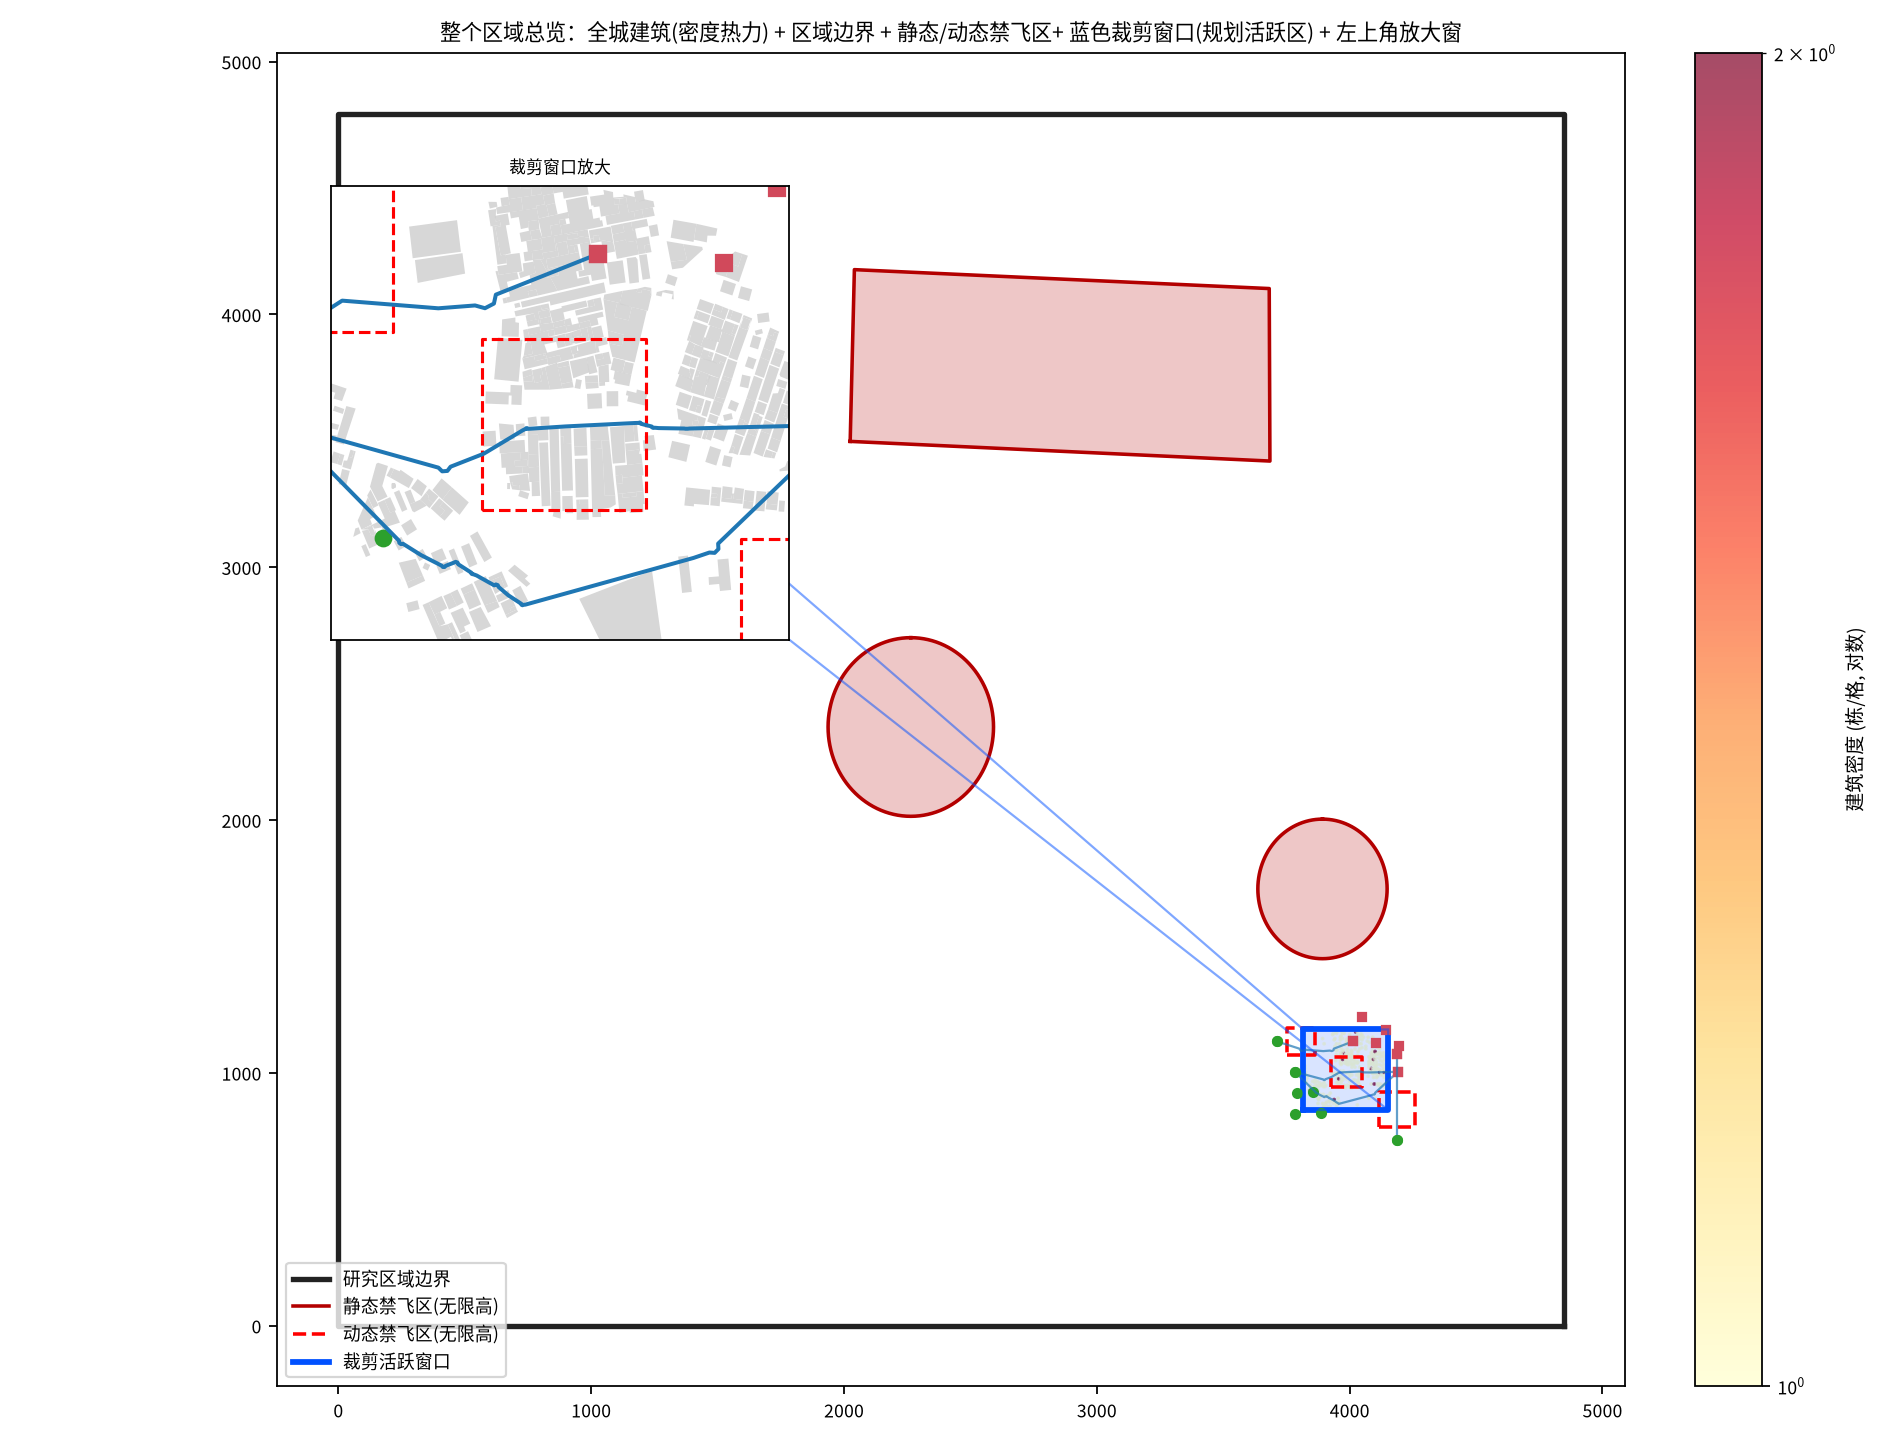
\includegraphics[width=0.92\textwidth]{fig_region_overview.png}
  \caption{整个区域总览：全城建筑密度热力 + 研究区边界 + 静/动态禁飞区 +
  裁剪活跃窗口（蓝框）+ 规划路径；左上角放大窗为裁剪窗口内细节。}
\end{figure}

\begin{figure}[H]\centering
  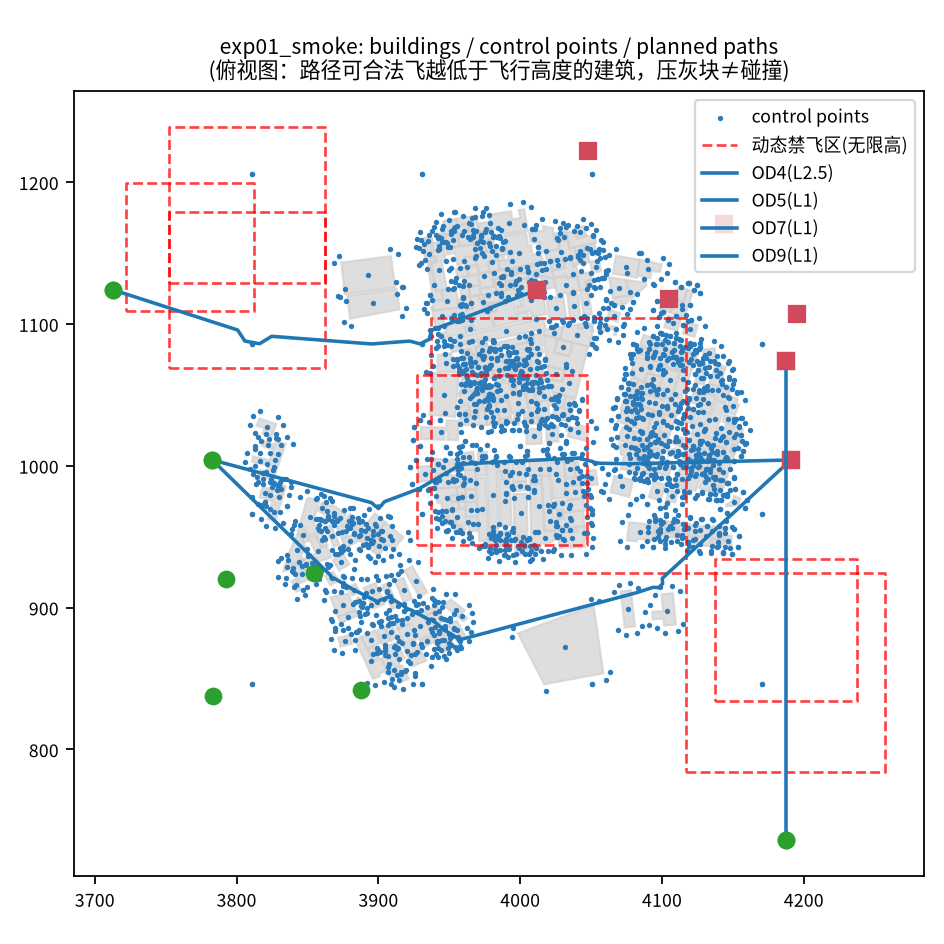
\includegraphics[width=0.62\textwidth]{fig_overview.png}
  \caption{场景俯视：建筑（灰）/ 控制点（蓝散点）/ 平滑路径。注意路径可合法飞越
  低于飞行高度的建筑，压灰块 $\ne$ 碰撞（碰撞结论以 audit 字段为准）。}
\end{figure}

\begin{figure}[H]\centering
  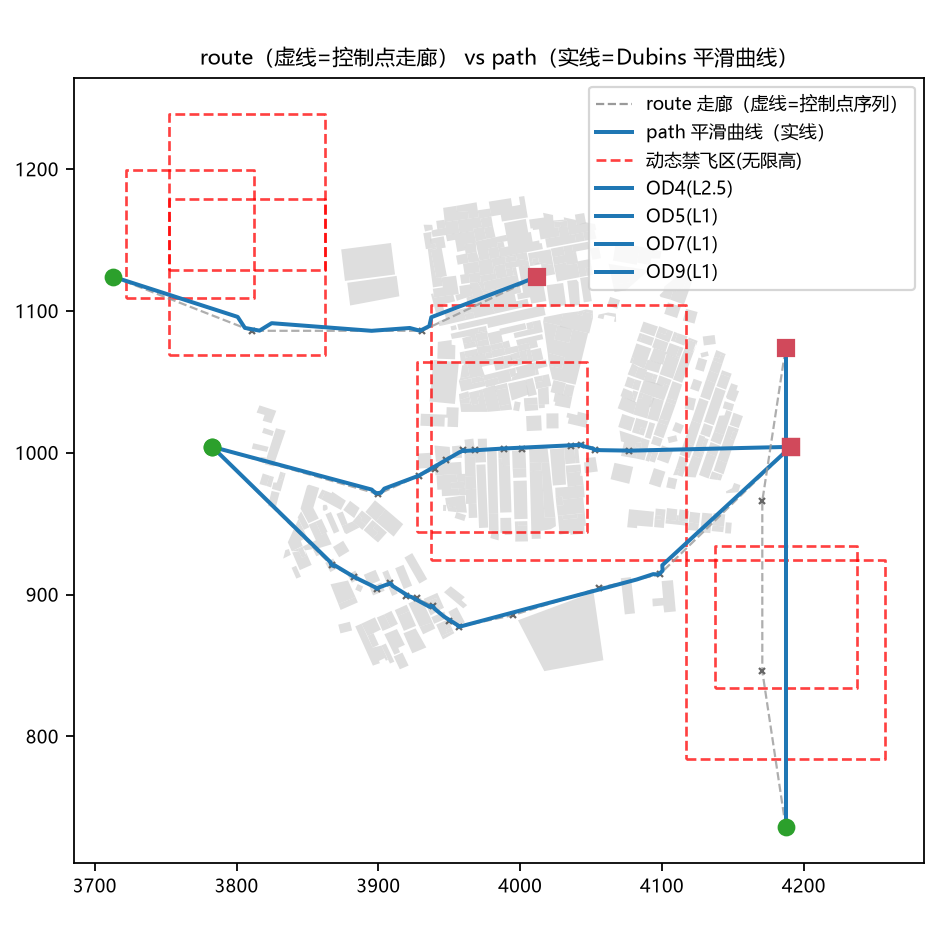
\includegraphics[width=0.62\textwidth]{fig_route_vs_path.png}
  \caption{route（灰虚线=控制点走廊）vs path（蓝实线=Dubins 平滑曲线）：
  两者几何口径严格区分，对应 Lin2021 Fig.1(a)(b)。}
\end{figure}

\begin{figure}[H]\centering
  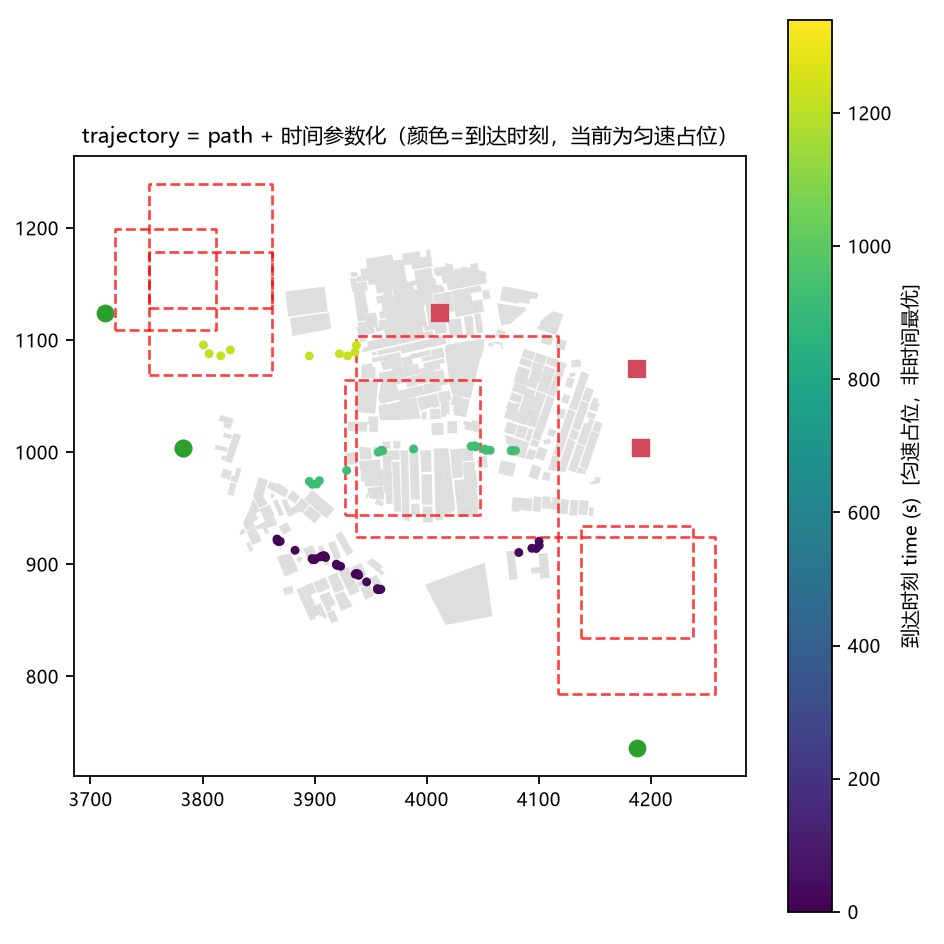
\includegraphics[width=0.62\textwidth]{fig_trajectory.png}
  \caption{trajectory = path + 时间参数化（颜色=到达时刻）。当前时间为匀速占位，
  非时间最优轨迹（time\_optimal.py 待实现）。}
\end{figure}

\begin{figure}[H]\centering
  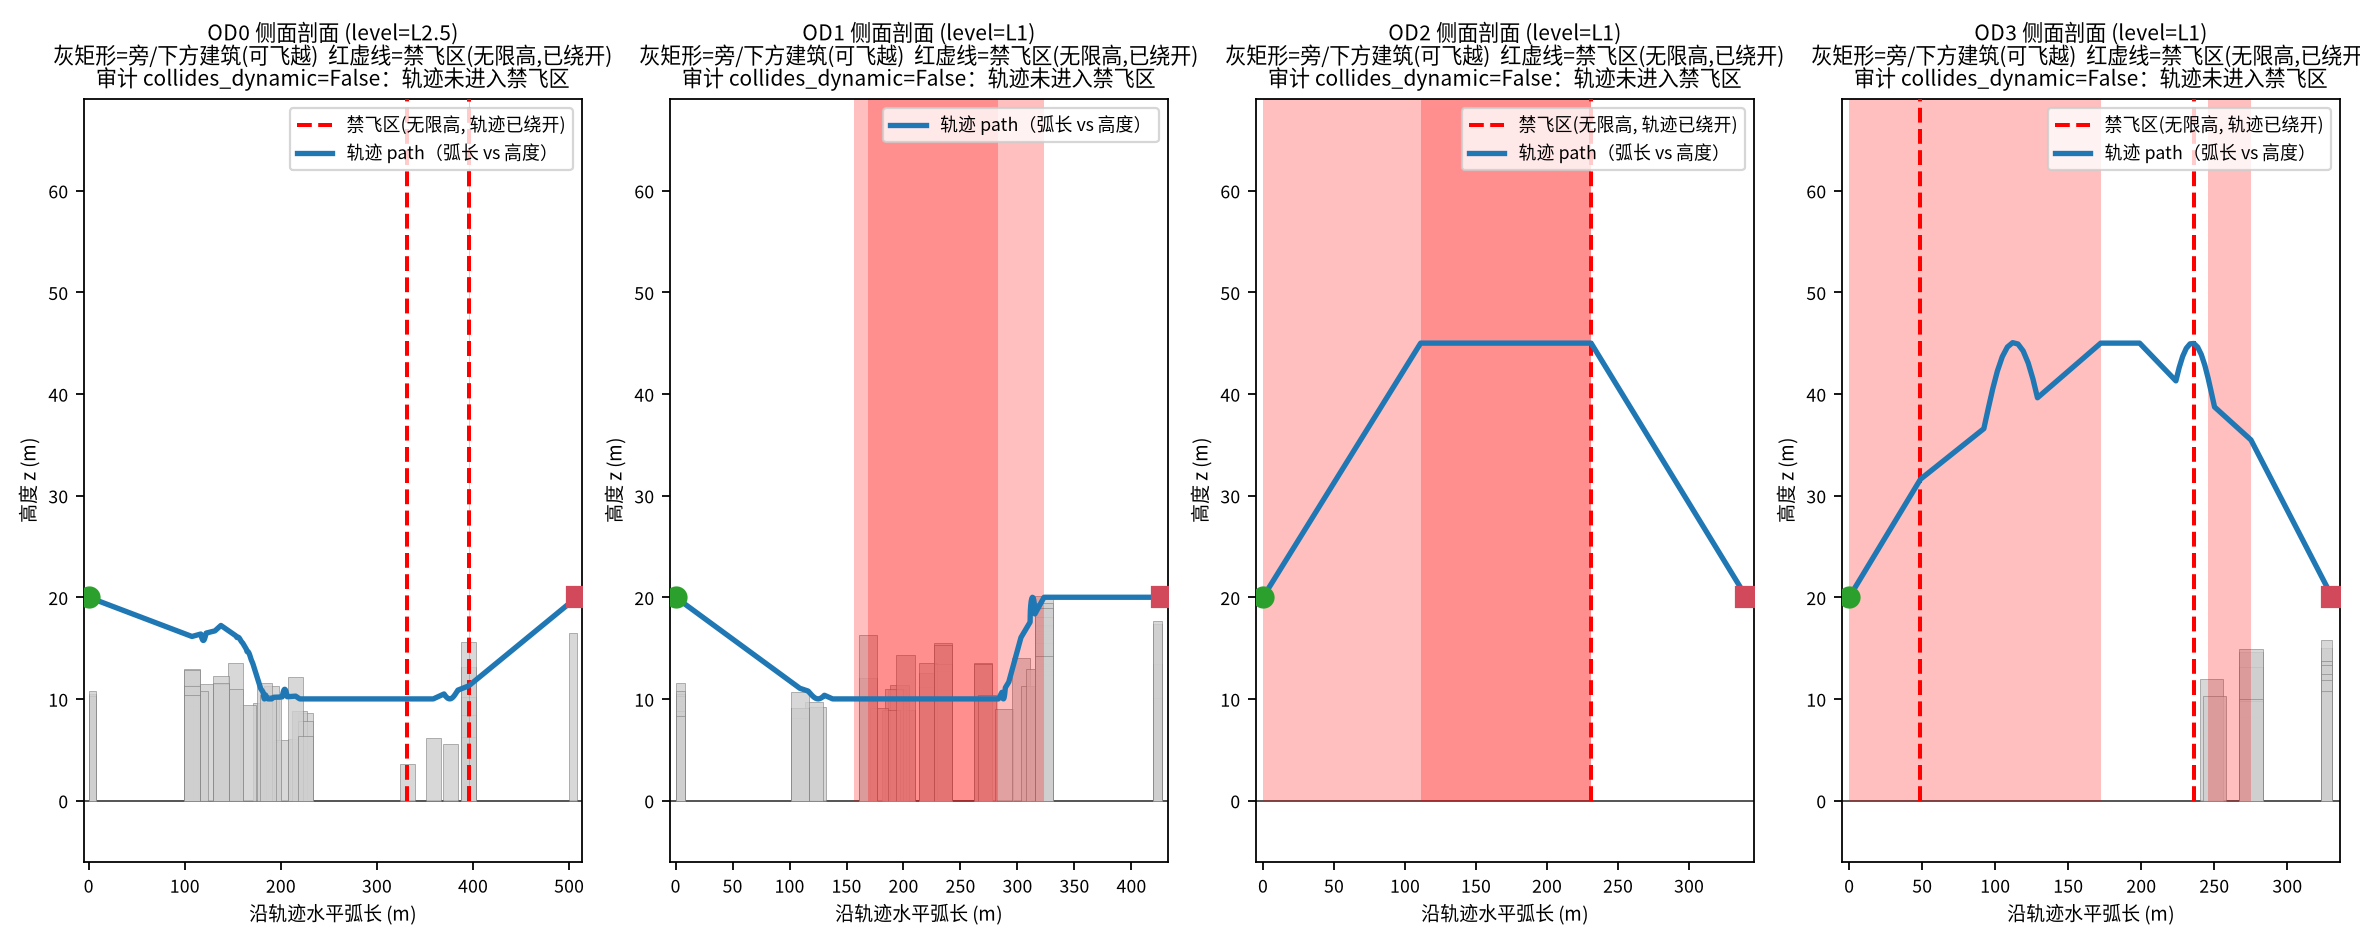
\includegraphics[width=0.92\textwidth]{fig_side_view.png}
  \caption{竖直剖面（弧长-高度）：灰矩形=轨迹近旁建筑（可飞越）；
  红虚线=无限高禁飞区约束参照（轨迹已横向绕开，未真实进入）。}
\end{figure}

\section{结论与已知限制}

\begin{enumerate}
  \item U1--U5 正确性用例全部通过；route/path/trajectory 三者口径在指标与图件中
        严格分存；独立复核（与搜索判定解耦的零余量"地面真值"）4/4 无碰撞。
  \item 动态禁飞按时间窗生效：同端点 OD 在时段内阻断、时段外 L1 可行（3/3），
        判定与恢复均正确；L2.5 保守全剪能在时段内找到绕行 route。
  \item \textbf{已知限制}：(a) trajectory 时间为匀速占位，非 §2.4 时间最优；
        (b) $\lambda_r=0$，TPR 风险项为论文保留章节未启用；
        (c) 本实验为正确性冒烟，样本量与统计口径留给 exp02/03。
  \item \textbf{本轮修复记录}（2026-10-29）：
        (i) 诊断 OD 端点原会越出裁剪窗口/贴边落入控制点稀疏带
        （\texttt{ORIGIN/DEST\_UNREACHABLE}），改为按禁飞区包围盒选横穿轴、
        端点离区 30--150\,m 且离窗口边留余量；
        (ii) \texttt{route\_search} 不可达原因语义修正：几何上吸附不到控制点才是
        \texttt{ORIGIN/DEST\_UNREACHABLE}，几何可达但接入段撞动态禁飞报
        \texttt{DYNAMIC\_BLOCKED}（时窗问题，换起飞时刻可解，原语义会误导闭环重调度）；
        (iii) 图件统一由 \texttt{plot/} 包产出（registry 图清单 + theme 学术样式，
        CJK 字体链修掉 Linux 豆腐块），落盘 \texttt{results/figures/}。
\end{enumerate}

\end{document}
